\documentclass[10pt,letterpaper]{article}
\usepackage[top=1in,bottom=1in,left=1in,right=1in]{geometry}
\usepackage{datetime}
\usepackage{natbib}      % http://merkel.zoneo.net/Latex/natbib.php
\usepackage{palatino}
\usepackage{verbatim}
\usepackage[normalem]{ulem}
\bibpunct{(}{)}{;}{a}{,}{,}

\usepackage{array}

\usepackage{chngpage}
\usepackage{stmaryrd}
\usepackage{amssymb}
\usepackage{amsmath}
\usepackage{graphicx}
\usepackage{lscape}
\usepackage{subfigure}
\usepackage[usenames,dvipsnames]{color}
\definecolor{myblue}{rgb}{0,0.1,0.6}
\definecolor{mygreen}{rgb}{0,0.3,0.1}
\usepackage[colorlinks=true,linkcolor=black,citecolor=mygreen,urlcolor=myblue]{hyperref}

\newcommand{\bocomment}[1]{\textcolor{Bittersweet}{BO says: #1}}

\newcommand{\ignore}[1]{}
\newcommand{\transpose}{^\mathsf{T}}
\newcommand{\inner}[1]{\langle #1 \rangle} 
\newcommand{\smallsec}[1]{\noindent \textbf{#1\ }}
\newcommand{\cmd}[1] {{\color{blue}\texttt{#1}}}

\newcommand{\solution}[1]{{\color{myblue} \emph{[Solution:} 
#1 

\emph{End solution]}}}
\newcommand{\solutionnote}[1]{{\color{myblue} \emph{[Note:}

#1 

\emph{End note]}}}
\newcommand{\points}[1]{{\color{mygreen}\emph{[#1]\ \ }}}

\newcommand{\aone}{\diamondsuit}
\newcommand{\atwo}{\heartsuit}
\newcommand{\bone}{\triangle}
\newcommand{\btwo}{\Box}
\newcommand{\myand}{\ \land\ }
\newcommand{\myor}{\ \lor\ }
\newcommand{\mynot}{\lnot}

\title{
  \textbf{Mini-project 4} \\
  \Large{CMPSCI 670, Fall 2019, UMass Amherst} \\
  \Large{Instructor: Subhransu Maji} \\
  \Large{TAs: Aruni RoyChowdhury, Archan Ray}
}

\settimeformat{ampmtime}
\date{}
\begin{document}
\maketitle

\renewcommand\thesubsection{\thesection.\alph{subsection}}


\section*{Guidelines}

\paragraph{Submission.} Submit a \emph{single pdf document} via moodle that includes your solutions, figures and code. The latex source file for the homework is provided which you can modify to produce your report. You are welcome to use other typesetting software as long as the final output is a pdf. For readability you may attach the code printouts at the end of the solutions within the same pdf. Note that we will not run your code. Similarly figures should be included in a manner which makes it easy to compare various approaches. Poorly written or formatted reports will make it harder for the TA to evaluate it and may lead to a partial deduction of credit. 

\paragraph{Late policy.} You could have 24 hours late submission with a 50\% mark down. Late submission beyond 24 hours will not be given \emph{any} credits.

\paragraph{Plagiarism.} We might reuse problem set questions from previous years, covered by papers and webpages, we expect the students not to copy, refer to, or look at the solutions in preparing their answers. We expect students to want to learn and not google for answers. 

\paragraph{Collaboration.} The homework must be done individually, except where otherwise noted in the assignments. 'Individually' means each student must hand in their own answers, and each student must write their own code in the programming part of the assignment. It is acceptable, however, for students to collaborate in figuring out answers and helping each other solve the problems. We will be assuming that you will be taking the responsibility to make sure you personally understand the solution to any work arising from such a collaboration.

\paragraph{Using other programming languages.} All of the starter code is in Matlab which is what we expect you to use. You are free to use other languages such as Octave or Python with the caveat that we may not be able to answer or debug non Matlab questions.

\paragraph{Python requirements.} We will be using Python 2.7. The Python starter code requires \cmd{scipy}, \cmd{numpy} (at least v1.12), \cmd{scikit-image} and \cmd{opencv-python}.
If you are not familiar with installing those libraries through some package manager (like \cmd{pip}), the easiest way of using them is installing \href{https://conda.io/docs/user-guide/install/index.html}{Anaconda}.
If you are using \cmd{pip}, you probably want to install \cmd{opencv-python} and \cmd{opencv-python-contrib} at the same time:
\\
\cmd{pip install opencv-python==3.3.0.10 opencv-contrib-python==3.3.0.10}.

\newpage

\section{Scale-space blob detection [45 points]}


\begin{figure}[h]
\centering
\begin{tabular}{cc}
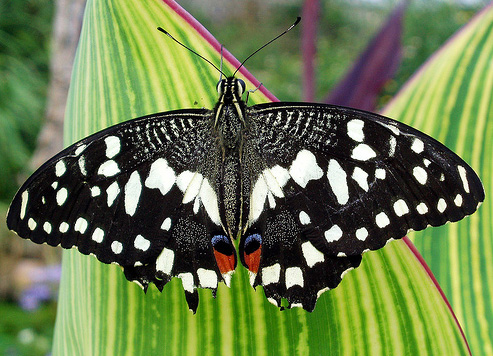
\includegraphics[width=0.4\linewidth]{./fig/butterfly.jpg} &
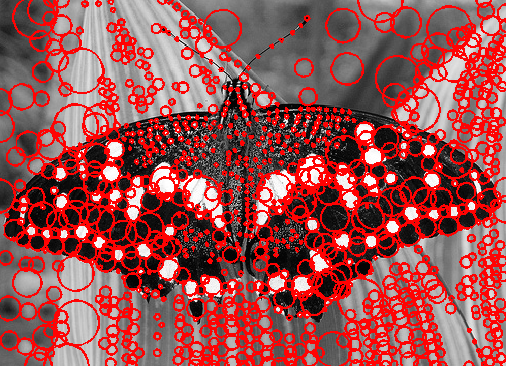
\includegraphics[width=0.4\linewidth]{./fig/butterfly.png} \\
\end{tabular}
\caption{\label{fig:blobs} Scale-space blobs detection}
\end{figure}


In this homework you will implement a simple panoramic image stitching algorithm. The first part is to detect blobs as keypoints. The algorithm is outlined as follows:

\begin{enumerate}
\item Build a Laplacian scale space, starting with some initial scale and going for n iterations:
\begin{enumerate}
\item Filter image with scale-normalized Laplacian at current scale.
\item Save the square of Laplacian response for current level of scale space.
\item Increase scale by a factor k.
\end{enumerate}
\item Perform non-maximum suppression in scale space.
\item Display resulting circles at their characteristic scales for points above a threshold.
\end{enumerate}

\paragraph{Test images.} There are four images in the folder \cmd{data/blobs} to test your code. Fig.~\ref{fig:blobs} provides the output of "butterfly" example as a reference to debug your code. Keep in mind that your output may look different depending on your threshold, range of scales, and other implementation details.

\paragraph{Running the code.} Start from the entry code \cmd{evalBlobsDetection}. It calls the dummy implementation of \cmd{detectBlobs} and draws the blob with \cmd{drawBlobs} as Fig.~\ref{fig:dummy}. You need to implement the detail in \cmd{detectBlobs} which outputs a $n \times 4$ matrix with a blob in each row as (x, y, radius, score). 

\begin{figure}[h]
\centering
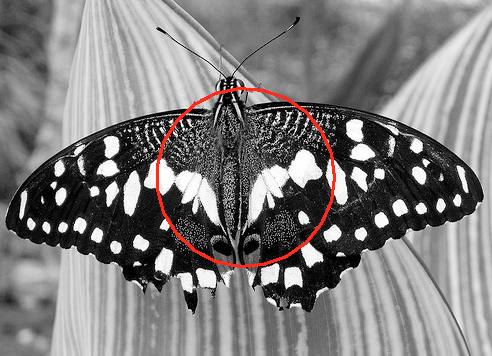
\includegraphics[width=0.3\linewidth]{./fig/butterfly-dummy.png} 
\label{fig:dummy}
\caption{\label{fig:dummy} Output of running the default implementation of evalBlobsDetection}
\end{figure}

The following are the hints to implement the function:

\begin{itemize}
\item Don't forget to convert images to grayscale (\cmd{rgb2gray} command) and double (\cmd{im2double}).
\item For creating the Laplacian filter, use the \cmd{fspecial} function (check the options). Pay careful attention to setting the right filter size.
\item You have to choose the initial scale, the factor $k$ by which the scale is multiplied each time, and the number of levels in the scale space. I typically set the initial scale to 2, and use 10 to 15 levels in the scale pyramid. The multiplication factor should depend on the largest scale at which you want regions to be detected.
\item You may want to use a 3D array to represent your scale space. It would be declared as:

\begin{center}
\textit{scaleSpace = zeros(h,w,n); \% [h,w] - dimensions of image, n - number of levels in scale space}
\end{center}

Then \textit{scaleSpace(:,:,i)} would give you the i'th level of the scale space. Alternatively, if you are storing different levels of the scale pyramid at different resolutions, you may want to use a cell array, where each "slot" can accommodate a different data type or a matrix of different dimensions. Here is how you would use it:
\begin{center}
\textit{scaleSpace = cell(n,1); \%creates a cell array with n "slots"} \\
\textit{scaleSpace\{i\} = myMatrix; \% store a matrix at level i}
\end{center}

\item A point is the local maximum if it is higher than all its neighbors (each point has 26 neighbors in 3D). You may find functions \cmd{nlfilter}, \cmd{colfilt} or \cmd{ordfilt2} useful for doing non-maximum supression in Matlab. In Python, you might want to use \cmd{scipy.ndimage.filters.generic\_filter} in your implementation.

\item You also have to set a threshold on the squared Laplacian response above which to report region detections. You should play around with different values and choose one you like best.

\item To display the detected regions as circles, you can use the \cmd{drawBlobs} function. You should display the highest scoring 1000 detected blobs for each image. If your code returns fewer than 1000 blobs then you may have to lower your threshold. Don't forget that there is a multiplication factor that relates the scale at which a region is detected to the radius of the circle that most closely approximates the region.
\end{itemize}

\subsection{What to submit}
To get full credit of this part, you have to
\begin{itemize}
\item Include your implementation of \cmd{detectBlobs} and include the results of given test images under \texttt{data/blobs}.
\end{itemize}


\section{Image stitching [35 points]}

In this part you will implement the RANSAC algorithm to stitch two images. The input to the algorithm are two images which are related by an unknown transformation. You will use your blobs detector implemented in the first part to extract keypoints and extract feature descriptors on them.  Your goal is to estimate an affine transformation using feature matching and RANSAC to produce a combined image. 


Recall that the overall steps in the alignment algorithm are:
\begin{enumerate}
\item Detect keypoints in each image (part 1).
\item Extract SIFT features at each detected keypoints.
\item Match features based on pairwise distance.
\item Use RANSAC to estimate the best affine transformation.
\item Stitch the two images using the estimated transformation.
\end{enumerate}

The provided codebase contains an implementation of Step 2 and Step 5. You will implement the remaining steps. The entry code for this homework is in \cmd{evalStitching}.  The code loads two images which contain overlapping areas. Figure~\ref{fig:inputs} shows the "hill" example included in the homework. More test examples are given in the \cmd{data/stitching} folder compressed in \cmd{p4\_data.zip}.


\begin{figure}[h]
\centering
\begin{tabular}{cc}
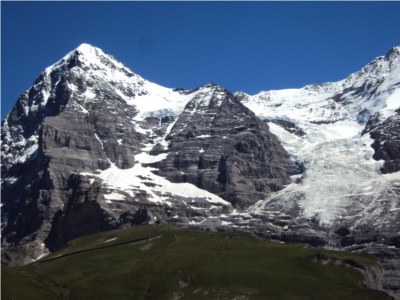
\includegraphics[width=0.45\linewidth]{./fig/hill1.jpg} &
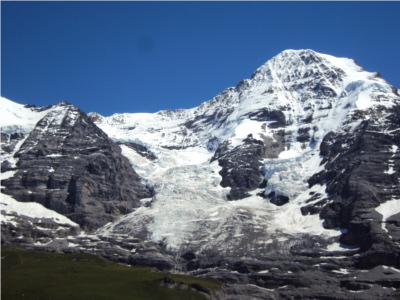
\includegraphics[width=0.45\linewidth]{./fig/hill2.jpg} \\
\end{tabular}
\caption{\label{fig:inputs} Input images to the image stitching algorithm.}
\end{figure}


Below is an outline of the steps you need to implement the algorithm.

\begin{enumerate}

\item \textbf{[0 points] Detect keypoints} The first step is to detect blobs in each image independently. You already implemented this in the first part. Remember to set the initial scale and threshold accordingly to get enough keypoints.
      
\item \textbf{[0 points] Feature extraction.} The next step is to extract feature descriptors on detected keypoints. The code to compute SIFT is included in the code base. The file \cmd{compute\_sift} takes an image and (x, y, radius) of $N$ blobs as input and return a matrix of size $N \times 128$ with 128 dimensional SIFT descriptor in each row. If you are using Matlab, the function uses different external libraries which are included in \cmd{mex} folder depending on the operating system. The first few lines in \cmd{evalStitching.m} sets up the environment variables in Matlab based on your operating system. The code has been tested to work on MATLAB 2019a version and earlier, and should work out of the box on Windows, MAC, and Linux platforms. Talk to the TA in case the mex files are not compatible with your operating system. If you are using Python, just install \cmd{opencv} using your favorite package manager.

\item \textbf{[10 points] Computing matches.} The next step is to compute matches between the two sets of features. Implement the function \cmd{matches = computeMatches(f1,f2)} that returns the best match of each feature \cmd{f1} to \cmd{f2} using the smallest sum-of-squared-differences. The input are two matrices \cmd{f1=dxN} and \cmd{f2=dxM} and the output is a array of size \cmd{Nx1} where each entry \cmd{matches(i)$\in$ [0,1,$\dots$,M]} is the closest feature in \cmd{f2} to the $i^{th}$ feature \cmd{f1(:,i)}, with \cmd{matches(i) = 0} indicating no matching (using MATLAB's 1-starting indexing; for Python a no-match can be indicated by -1).

Considering only nearest neighbors returns many false matches. To refine the matches, compute the ratio of distance from the closest feature to the distance from the second closest feature and reject the matches with the ratio greater than a threshold. \href{http://www.cs.ubc.ca/~lowe/papers/ijcv04.pdf}{David Lowe's paper} suggest a threshold 0.8. Set \cmd{matches(i)=0} if $i^{th}$ feature \cmd{f1(:,i)} fails on the ratio test.

You can visualize the matches using the \cmd{showMatches(im1, im2, c1, c2, matches)} function provided in the codebase. Figure~\ref{fig:match} shows the output of my implementation for reference.

\begin{figure}[h]
\centering
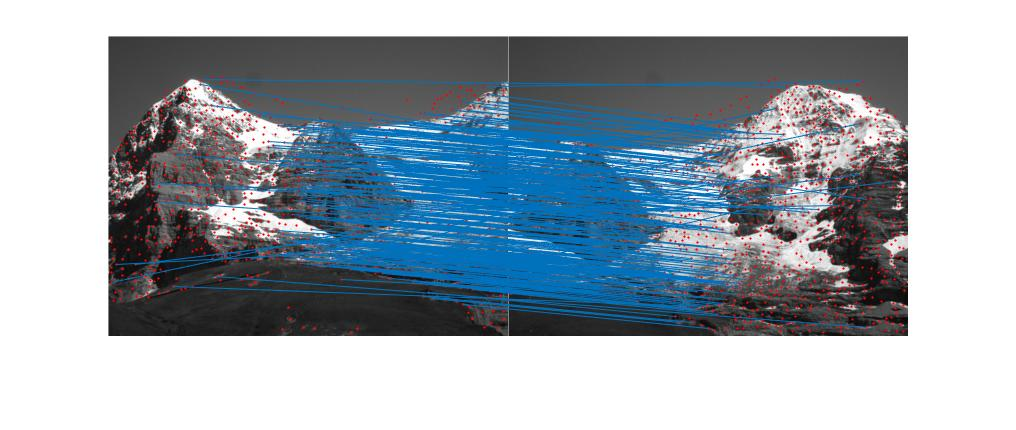
\includegraphics[width=0.95\linewidth]{./fig/matched.jpg}
\vspace{-0.6in}
\caption{\label{fig:match} Matches between features.}
\end{figure}

\item \textbf{[25 points] Estimating affine transformation using RANSAC.} The matching in the previous step is noisy and contains many outliers. Using RANSAC, estimate the affine translation that agrees with most matches (inliers). Implement the function \cmd{[inliers, transf] = ransac(matches, c1, c2)}. Here inliners is the indices of the inliner matches, transf is the estimated affine translation of $2\times 3$ matrix \cmd{$[m_1, m_2, t_1; m_3, m_4, t_2]$} between c1 and c2 (See the notation in Lecture slides). You need at least three pairs of points to estimate the this. See lecture slides for details.

You can visualize the inlier matches using the \cmd{showMatches} function. Figure~\ref{fig:ransac_result} shows the output of my implementation for reference. The estimated affine transformation for this example is given as follows for your reference:

\begin{center}
$\begin{bmatrix}
0.9827 &  0.1855 & 124.1568 \\
-0.1782 & 0.9804 & 0.9023 \\
\end{bmatrix}$
\end{center}

\begin{figure}[h]
\centering
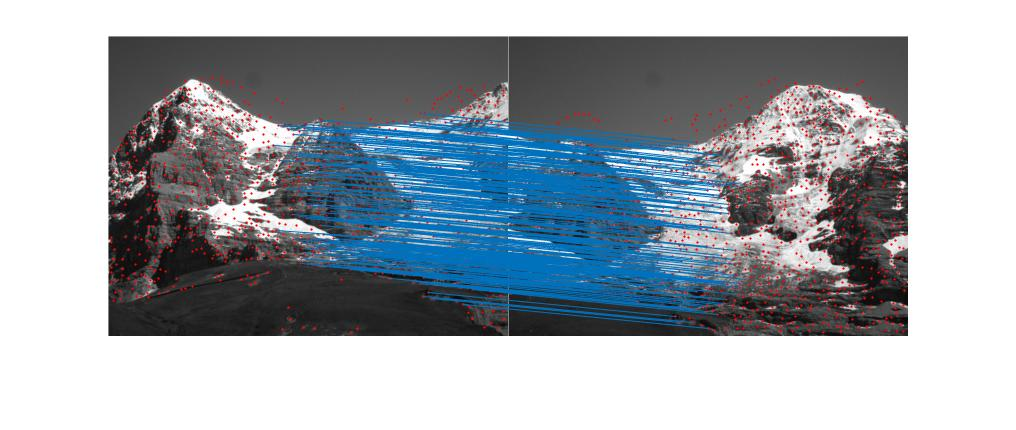
\includegraphics[width=0.95\linewidth]{./fig/ransac_result.jpg}
\vspace{-0.6in}
\caption{\label{fig:ransac_result} Inliers obtained from RANSAC.}
\end{figure}

\begin{figure}[h]
\centering
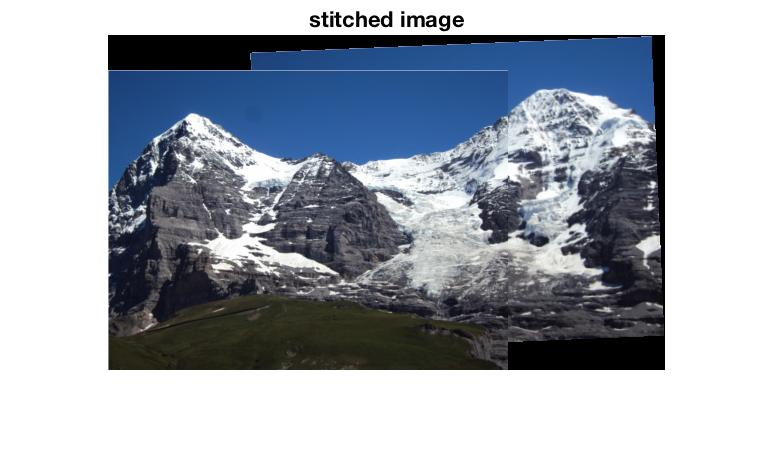
\includegraphics[width=0.8\linewidth]{./fig/stitch_result.jpg}
\vspace{-0.6in}
\caption{\label{fig:output} Visualization of output.}
\end{figure}
\item \textbf{[0 points] Visualizing the stitched image.} Merge the images using \cmd{mergeImages(im1,im2, transf)} function provided in the codebase. The result is shown as Figure~\ref{fig:output}.
\end{enumerate}



 
\subsection{What to submit}
To get full credit for this part you have to
\begin{itemize}
\item Include your implementation of \cmd{computeMatches.m} and \cmd{ransac.m}.
\item Visualize the intermediate results and the output of each of the provided test image pairs. You can do this by setting the \cmd{exampleIndex} variable in the \cmd{evalStitching.m} file.
\item Report the estimated affine transformation for given test images.
\end{itemize}


\section{Report Writing and Presentation [10 points]}
Please follow the guidelines for writing a good report. Graders will penalize reports that are poorly written and fail to present the results in a reasonable manner

\vspace{-0.1in}
\section{Extensions for extra credit}
\begin{itemize}
\item To detect blobs at multiple scales, there are two strategies to complete the task: (1) iteratively filter the image with kernel of increasing size. (2) iteratively downsample the image and filter it with the kernel of fixed size. You will have to upsample the result or do some interpolation in order to find maxima in scale space for the second approach. Which approach is more efficient? Run the both implementations and compare the performance between them.

\item Implement the difference-of-Gaussian pyramid as mentioned in class and described in \href{http://www.cs.ubc.ca/~lowe/papers/ijcv04.pdf}{David Lowe's paper}. Compare the results and the running time to the direct Laplacian implementation.

\item Implement the affine adaptation step to turn circular blobs into ellipses as shown in the lecture. The selection of the correct window function is essential here. You should use a Gaussian window that is a factor of 1.5 or 2 larger than the characteristic scale of the blob. Note that the lecture slides show how to find the relative shape of the second moment ellipse, but not the absolute scale (i.e., the axis lengths are defined up to some arbitrary constant multiplier). A good choice for the absolute scale is to set the sum of the major and minor axis half-lengths to the diameter of the corresponding Laplacian circle. To display the resulting ellipses you should modify the circle drawing function or look for a better function in the MATLAB or on the Internet.

\item The Laplacian has a strong response not only at blobs, but also along edges. However, recall from the class lecture that edge points are not "repeatable". So, implement an additional thresholding step that computes the Harris response at each detected Laplacian region and rejects the regions that have only one dominant gradient orientation (i.e., regions along edges). If you have implemented the affine adaptation step, these would be the regions whose characteristic ellipses are close to being degenerate (i.e., one of the eigenvalues is close to zero). Show both "before" and "after" detection results.

\item There are few difficult test images where affine transformation will not produce perfect results since some 2D transformations cannot be modeled as affine (See section 2.1 in \href{http://szeliski.org/Book/drafts/SzeliskiBook_20100903_draft.pdf}{Richard Szeliski's book}). For example, you could to align two images with a homography.
\end{itemize}
If you complete any work for extra credit, be sure to clearly mark that work in your report, explain it and include the code.



\end{document}
